%%This is a modified IEEE format for ReVeCom
\documentclass[10pt]{revecom}

% Some very useful LaTeX packages include:
% (uncomment the ones you want to load)


\ifCLASSINFOpdf
  \usepackage[pdftex]{graphicx}
\else
  \usepackage[dvips]{graphicx}
\fi

\usepackage{multirow}
\usepackage{multicol}

\usepackage{cite}
\usepackage{amsmath,amssymb,amsfonts}
\usepackage{algorithmic}
\usepackage{graphicx}
\usepackage{textcomp}
\usepackage{xcolor}
\usepackage{minted}


\usepackage{amssymb}
\usepackage[spanish]{babel}	%Incluye caracteres del español
\usepackage{amsmath}		%Funciones matemáticas
\usepackage{graphicx}		%Gráficas
\usepackage{dcolumn}
\usepackage{hyperref}
\usepackage[utf8]{inputenc}	%Permite añadir tildes al documento

\usepackage{flushend}
% Para empatar las dos columnas de la ultima pagina

\usepackage{enumitem}
\setlist[itemize,1]{leftmargin=0.25in}
% Para la identacion de las listas de balas (bullet lists o itemize)

%\usepackage[draft]{hyperref}
% Para los URLs


\usepackage{balance}

% correct bad hyphenation here
\hyphenation{op-tical net-works semi-conduc-tor}


\begin{document}
\newcommand*{\nextpar}{\vspace{6.0pt}} % separation of paragraphs
\pagenumbering{gobble}  % turn off page numbering

\twocolumn[
\begin{@twocolumnfalse}


\vspace{3pt} \noindent
\begin{tabular}{|p{508pt}|}
\hline \vspace{-0.1cm}
\parbox{508pt}{\centering {\fontsize{20}{24}\selectfont
Please, do not Remove this Frame }} \\
~ \vspace{0.5in} \\ \hline
\end{tabular}
\vspace{0.5cm}

\begin{center}
{\fontsize{20}{24}\selectfont
Manual-design of Blocks (MoB): Una Herramienta para Gestionar Segmentaciones Manuales de Páginas Web
}
\vspace{0.2cm}

%Jean Garcia$^{1}$, Andres Sanoja$^{1}$ \\
%jeangarcialunardi95@gmail.com, andres.sanoja@ciens.ucv.ve \\
%\vspace{0.4cm}

%$^{1 \:}$Escuela de Computaci\'on, Universidad Central de Venezuela,
%Caracas, Venezuela \\
%\vspace{0.2cm}
\end{center}



\begin{center}
\noindent\rule{510pt}{0.4pt}
\end{center}
\vspace{-0.1cm}

\begin{center}
\begin{minipage}{0.95\textwidth}
\textbf{Resumen:} 
La segmentación es una parte importante en el análisis de páginas Web. 
El objetivo es dividir una página en bloques, cada uno representando una parte (o segmento) coherente del contenido.
%
%Comparar segmentaciones es una tarea compleja. Los modelos de analisis de páginas son basados en heurísticas. Para una evaluación efective se requiere un modelo formal, el cual, en nuestro conocimiento, no esta disponible ni implementado en los motores de renderizado.
En el presente trabajo describimos el desarrollo de la herramienta Manual-design of Blocks (MoB).
Se incluyen detalles de la investigación, donde se comprueba la importancia de MoB en la evaluación de algoritmos de segmentación. 
El objetivo de nuestro trabajo es el desarrollo de la herramienta MoB. Al mismo tiempo describir los mecanismos para la obtención de una ``base referencial''\footnote{En inglés ``Ground truth'', refiere a una colección de datos que generan la información la cual es usada de referencia para futuras operaciones} de segmentaciones manuales sobre una misma página y para la posterior obtención de ``la mejor segmentación manual''. 
La mejor segmentación manual es definida en base a nuestra experiencia y los datos obtenidos, en este trabajo se define una forma de su obtención pero no se considera que sea la única forma de obtener.La mejor segmentacón obtenida queda disponible para la evaluación de un algoritmo de segmentación usando el framework Block-o-Matic. 
Mediante el uso de MoB se soporta el proceso de conformación de la base referencial, apoyado con una interfaz de programación de aplicaciones Web (API) y un repositorio para su manejo y consulta.
Se presentan resultados de las pruebas de aceptación. 
\nextpar

\textbf{Palabras Clave:} segmentación, página web, segmentación manual, bom, block-o-matic
\nextpar

\textbf{Abstract:} 
Web page segmentation is an important task in Web page analysis. The objective is to divide a Web page into blocks, each one representing a coherent part (or segment) of the content. 
In this work we describe the development of the Manual-design of Blocks (MoB). At the same time we describe how to get a ground truth of segmentations and how to compute the``best manual segmentation''.
The best manual segmentation is defined based on our experience and the data obtained, in this investigation we define one way to obtain it, but we do not consider there's only one way to achieve this. The best segmentation is then available to be used on the evaluation process of segmentation algorithm using the Block-o-Matic framework. 
Also, a Web API and a Web repository for managing the data.
Acceptance test results are presented in this document.
\nextpar

\textbf{Keywords:} segmentation, web page, manual segmentation, bom, block-o-matic
\end{minipage}
\end{center}
\vspace{-0.1cm}
\begin{center}
\noindent\rule{510pt}{0.4pt}
\end{center}

\end{@twocolumnfalse} ]

\section{Introducción}
La página Web es un documento digital de información accesible mediante un navegador de Internet.
Esta información se presenta generalmente en formato HTML. 
Está compuesta por un conjunto de elementos ordenados en una estructura de árbol (el árbol DOM), generado por el navegador a partir del código fuente HTML \cite{Zhu:18:WD}.
%
En el caso del presente trabajo, la segmentación de una página Web es la acción de dividir una página Web en fragmentos coherentes (\emph{i.e} cada fragmento debe tener un sentido para un usuario) llamados bloques \cite{Sanoja:LIP6:2015}. 
%
Cada bloque representa distintos elementos de información en la página. 
%
Un algoritmo de segmentación define las reglas para la selección de dichos segmentos. En general, estas reglas se definen en base al árbol DOM y las pistas visuales, \emph{e.g.} tamaño de la letra, separación, espaciado o colores.
%
Otros enfoques se definen en base a \emph{screenshots} o el texto de una página.
%
La segmentación puede ser aplicada en diferentes áreas como por ejemplo: 
\begin{itemize}
\item \textbf{Procesos de SEO o \textit{Search Engine Optimization}}. La segmentación de la página Web permite realizar un análisis del contenido de la página para que esta pueda ser calificada y ubicada en un \emph{ranking}.
%
\item \textbf{Migración de Formatos}. La segmentación de la página Web puede ser utilizada para ayudar en el proceso de conversión del formato de un documento a otro diferente. Por ejemplo, se puede migrar una página Web de la versión del lenguaje HTML4 a HTML5. Se convierten los bloques de la página en HTML4 a elementos semánticos, los cuales se utilizan para la creación de la nueva versión de la página usando el lenguaje HTML5 (\emph{e.g.} section, article). 
%
\item \textbf{Archivado de la Web o Web Archiving}. La segmentación permite comparar dos versiones de la misma página Web, la versión que actualmente se tiene almacenada y la versión que se planea almacenar. El encontrar las diferencias entre ellas permite detectar si resulta eficiente descargar y almacenar la nueva versión y sus dependencias. 
%
\item \textbf{Bloqueo de Contenido o \textit{Content Blocking}}. La segmentación de la página Web permite  identificar los segmentos dentro de la página que poseen contenido no deseado para ciertas audiencias. De esta manera bloquear solamente una porción de la página sin afectarla como a un todo.
\end{itemize}
%
Es importante considerar las necesidades de cada área, dependiendo de si se desea un algoritmo de segmentación genérico o un algoritmo de segmentación específico. 
Se entiende que mientras más genérico sea, podrá ser usado en mayor cantidad de páginas Web pero con menos precisión. 
%
Para poder precisar esto el algoritmo de segmentación debe ser evaluado \cite{SanGan:SAC:2015}. 
%
Esta evaluación se enfoca en comparar la segmentación obtenida con un algoritmo contra una segmentación denominada como ``la mejor segmentación manual''.
Así mismo con la conformación de una ``base referencial''. En ella residen las páginas previamente segmentadas y anotadas. Se utiliza para apoyar tanto la evaluación como la construcción de la mejor segmentación manual.
%
Definir un método de evaluación formal, en el alcance de nuestro conocimiento, no es práctico en base a la naturaleza de los estándares (\emph{ie} reglas heurísticas) W3C.
%
Consideramos una segmentación manual como la mejor opción para este caso.
%
Obviamente, esta técnica no sustituye un enfoque formal, ya que puede resultar subjetivo dependiendo de la visualización que posea el usuario \cite{Cai:APWEB:2003}. 
%
Buscamos la mejor segmentación manual, la cual es una composición basada en el consenso entre las diferentes segmentaciones realizadas por varios usuarios sobre una misma página Web y con la misma granularidad.
%
El principio es que un bloque estará en la mejor segmentación si el área de la página ha sido seleccionada por la mayoría de los usuarios como un bloque.
%
Ambas segmentaciones deben estar ajustadas a una misma granularidad, la cual define el tamaño general de los bloques dentro de una segmentación. Se define entonces, para nuestro caso, que la mejor segmentación manual es aquella que contiene los bloques más populares en un conjunto de segmentaciones manuales.
Si la mayoría de usuarios han marcado un área de la página como un bloque, este se considerará popular.
Entonces se toman los bloques más populares, se crea una nueva segmentación que los contenga, y esta será considerada la mejor. Más información acerca de la obtención de la mejor segmentación manual se describe en la sección IV-C.  

%
Segmentar una página Web manualmente puede ser una tarea compleja y propensa a errores. 
%
Un usuario debe tener conocimientos avanzados del lenguaje HTML y sus dependencias.
%

\textbf{Contribución}: 
El presente trabajo tiene como objetivo ofrecer una solución para la obtención de la mejor segmentación manual mediante el desarrollo de una herramienta que permite a cualquier usuario realizar segmentaciones manuales de páginas Web.
La solución incluye tres componentes: una extensión del navegador para la segmentación manual (MoB extension), una aplicación Web como \textit{endpoint} que recibe las segmentaciones manuales, construye la mejor segmentación manual y gestiona los datos (MoB API). Finalmente, un repositorio como archivo Web (MoB Repository).
Estan disponible MoB Repository y descargar la exensión de MoB desde el sitio Web \footnote{https://mob.ciens.ucv.ve/} o descargar el código fuente desde Github \footnote{https://github.com/JeanGarcia/MoB}. 

\textbf{Organización}: 
En la sección \ref{trabajos_referencia} presentamos los antecedentes. 
En la sección \ref{segmentacion_manual} describimos la herramienta de segmentación manual y consideraciones sobre la granularidad. 
En la sección \ref{api_repo} presentamos la API, el repositorio y la propuesta de como obtener la mejor segmentación manual. 
En la sección \ref{resultados} describimos la verificación funcional de la herramienta. 
En la sección \ref{conclusiones} presentamos las conclusiones y trabajos a futuro.

\section{Antecedentes}
\label{trabajos_referencia}
%Unlike its counterpart in the area of Computer Vision, manual segmentation tools for the Web have not been very popular.
%What is found, and is more common, is to annotate within the HTML code.
%In principle, this technique would allow us to indicate which elements belong to a block and assign it a label.
%However, it is a tedious, long and error-prone activity.
%Requires advanced knowledge of HTML and Web browsers.
%%
%Some solutions use manual segmentation as annotations and are very focused on measuring the \textit{precision} and \textit{recall} metrics, for example in \cite{liu2011segmenting, uzun2013hybrid}.
%Others focus on considering blocks as nodes of a graph in order to annotate pages with weights to apply clustering metrics, as is the case with \cite {Chakrabarti:WWW:2008,10.1145/3326457}.
%%
%It is in our interest to have a mechanism that allows, in a generic way, to manually segment any page to be used in an evaluation process and graphically.
%\ cite {kiesel-etal-2017-wat} present its version for segment tag annotation.
%Given a segmentation (in this case the blocks are sentences in a text), an expert provides the labels to each of the specified segments.


A diferencia de su contraparte en el área de Computación Gráfica, las herramientas de segmentación manual para la Web no han sido muy populares. Lo que si se encuentra, y es mas común, es realizar anotaciones dentro del código HTML. 
En principio esta técnica nos permitiría indicar cuales elementos pertenecen a un bloque y asignarle una etiqueta.
Sin embargo, es una actividad tediosa, larga y propensa a errores. Requiere conocimientos avanzado de HTML y sobre navegadores Web. 
Algunas soluciones utilizan la segmentación manual como anotaciones y son muy enfocadas en medir las
métricas de precision y recall, por ejemplo en \cite{liu2011segmenting, uzun2013hybrid}.
Otros se enfocan en considerar bloques como nodos de un grafo para así anotar páginas con pesos para aplicar métricas de clustering, como es el caso de \cite {Chakrabarti:WWW:2008,10.1145/3326457}. 

Es de nuestro interés contar con un mecanismo que permita de manera genérica, segmentar manualmente cualquier página para ser utilizado en un proceso de evaluación y de manera gráfica. Kiesel, Wachsmuth, Al-Khatib y Stein (2017)\cite{kiesel-etal-2017-wat} presentan su versión para anotación de etiquetas de segmentos. Dada una segmentación (en este caso los bloques son oraciones en un texto), un experto aporta las etiquetas a cada uno de los segmentos especificados.
%
Aun cuando en su trabajo se realiza una segmentación de texto (realizada sobre el texto de una página directamente), la herramienta WAT-SL, desarrollada a lo largo de su investigación, es en esencia similar a a la herramienta MoB, ya que también es usada para segmentar y anotar dichos segmentos con etiquetas.
Contiene apoyo gráfico y no está restringida a un conjunto de datos de prueba en particular.

Otros investigadores han trabajado también en la evaluación de segmentaciones de páginas Web, construyendo segmentaciones manuales para probar los evaluadores \cite{bjdmnmd2019,krh2015}. 
Estos últimos generaron \textit{datasets} para pruebas de sus tesis doctorales, que luego quedaron disponibles en línea. Utilizan elementos de CSS para denotar un bloque, mediante el uso de clases CSS.
Aun cuando es un enfoque interesante, deja de lado los aspectos geométricos inherentes de los elementos de una página Web. Siendo estos un elemento clave, común en todos los algoritmos de segmentación y así poder compararlos. 

Nuestro trabajo forma parte de la evaluación de la segmentación de páginas Web. 
Fue descrito como un trabajo futuro propuesto por Sanoja y Gançarski (2015) \cite{Sanoja:LIP6:2015,SanGan:SAC:2015}.
%
En el trabajo se presenta el uso del framework de segmentación de páginas Web Block-o-Matic (BoM), para migrar documentos en formato HTML4 a formato HTML5 para evitar la obsolescencia en el contexto de archivos Web.
%
BoM es la herramienta basada en el algoritmo homónimo \cite{Sanoja:ICMCS:2014}, para la segmentación de una página Web de forma automática. 
\emph{MoB-protoype} (Prototipo de Manual-design of Blocks) es la herramienta de segmentación manual, cuya versión debe ser mejorada.
Se utilizó como un prototipo de baja fidelidad implementado como una extensión para el navegador Chrome, llevando el proceso de manera semi-automática. Esta herramienta está orientada a usuarios expertos.

\begin{figure}[htbp]
\centerline{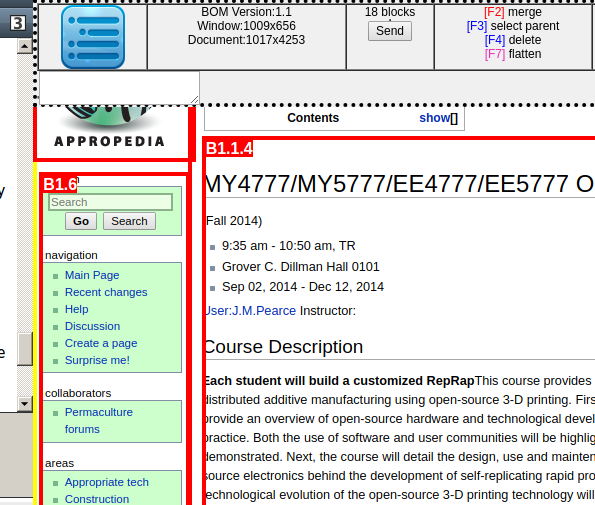
\includegraphics[width=250px]{old-mob.png}}
\caption{Versión prototipo de  \emph{MoB}}
\label{fig1}
\end{figure}

En la Figura \ref{fig1} se puede observar un ejemplo de como el usuario crea bloques dependiendo de los elementos del DOM. 
Se obtiene un grafo de bloques (respetando la jerarquía en el DOM) o simplemente una segmentación plana (sólo bloques terminales). 
Ambas segmentaciones se materializan en un documento XML. 
Produce también un conjunto de rectángulos presentados de manera visual.

En la Figura \ref{eq1} se observa que \emph{MoB-protoype} posee un panel en la parte superior.
En el panel se muestra la leyenda de los comandos a usar para realizar la segmentación manual. 
Se le presenta al usuario una segmentación realizada previamente por BoM. 
Se le propone al usuario aceptar o modificar la segmentación propuesta. 
Si el usuario desea modificar la segmentación, por ejemplo agregar un bloque, debe presionar F9 y hacer clic en el elemento que desea segmentar. 
Mediante el uso de las flechas del teclado el usuario puede navegar la jerarquía del DOM.

Una vez se hayan completado los pasos anteriormente mencionados, y el usuario escoja el elemento DOM que desea segmentar, se resaltará dicho elemento indicando que se ha segmentado.
Este proceso resulta tedioso, complicado y propenso a errores, incluso para usuarios expertos. 
Es recomendable realizar una mejora en la usabilidad de \emph{MoB-protoype}. 
Por ejemplo, resaltar tentativamente el elemento que se desea segmentar permitiéndole al usuario una retroalimentación activa y se crea también un sistema de puntajes, el cual motiva a los usuarios a realizar segmentaciones, entre otros aspectos a considerar.
Proponer una segmentación usando BoM al inicio puede no ser justo con otros algoritmos, por lo que se recomienda no utilizarlo.

En las siguientes secciones se presentaran las mejoras realizadas a \emph{MoB-protoype} en su nueva versión.

\section{Extensión MoB}
\label{segmentacion_manual}
La extensión de MoB es la herramienta de segmentación manual desarrollada por nosotros\footnote{Disponible en https://mob.ciens.ucv.ve}. Se utiliza Javascript, HTML5 y CSS3, como una extensión para navegadores Chrome y Chromium.

\subsection{Funcionalidades de la Extensión MoB}
\begin{itemize}
\item \textbf{Consultar información:} sección de información donde el usuario puede aprender más de la herramienta y sus diferentes acciones.
\item \textbf{Cambiar idioma:} permite al usuario cambiar el idioma de la interfaz escogiendo entre: inglés, francés o español. 
\item \textbf{Consultar puntuaciones:} permite a un usuario autenticado en el sistema consultar sus puntuaciones personales sobre una determinada página Web o las puntuaciones globales. 
\item \textbf{Registro:} permite al usuario registrarse dentro del sistema MoB.
\item \textbf{Autenticación:} una vez el usuario está registrado, el sistema le permite autenticarse mediante un inicio de sesión. 
\item \textbf{Segmentación manual:} el sistema le permite al usuario identificado inicializar la herramienta de segmentación manual.
\end{itemize}

\subsection{Acciones de la Herramienta de Segmentación}
A continuación describimos las acciones que ofrece la extensión MoB. 
Al inicializar la herramienta de segmentación manual, aparecerá un menú con las siguientes acciones: 
\begin{itemize}
\item \textbf{Agregar nuevo bloque:} agregar un nuevo bloque a la segmentación. 
Al ser seleccionada, el usuario puede recorrer los elementos del DOM con el ratón y estos serán iluminados.
Una vez el usuario haga clic sobre alguno de estos elementos del DOM, se insertará en el HTML un rectángulo representando el bloque segmentado. 
Este rectángulo posee entre sus atributos los datos del bloque segmentado (etiqueta, ancho, alto, posición horizontal, posición vertical y el área). 
Estos datos son almacenados dentro de un arreglo en Javascript. Este arreglo es utilizado para realizar las comparaciones necesarias entre los diferentes bloques para aplicar las  acciones. 
Al realizar esta acción se activa un subproceso que verifica si hay otros bloques dentro del que está a punto de crearse. 
De ser así se eliminan dichos bloques y se conserva únicamente el nuevo que ha sido creado. 
En caso de que existan bloques que se intersecten parcialmente con otros bloques, es necesario la acción de ``cortar'', \emph{i.e.} ajustar los rectángulos.
\item \textbf{Eliminar bloque:} una vez activada, se iluminaran aquellos bloques al que el usuario señale con el ratón. 
Al hacer clic sobre alguno de estos bloques se disparará una función de Javascript la cual removerá el elemento DOM que representa el rectángulo del bloque. Será removido del arreglo de bloques.
\item \textbf{Unir bloques:} al ser seleccionada, esta acción permite al usuario seleccionar dos bloques los cuales se unirán. 
Esta acción elimina los dos bloques seleccionados y crea uno nuevo que comparte los límites superiores e inferiores máximos de los bloques anteriores. 
Después se comprueba que no cubra otros bloques dentro del nuevo, en cuyo caso se eliminarían los internos.
\item \textbf{Cortar bloques:} esta acción permite seleccionar dos bloques que se solapen (A y B) y realizar un corte entre los dos. El orden de selección importa, pues A será el bloque que predominará (se mantendrá intacto) y B será el bloque que se recortará y ajustará.
\item \textbf{Etiquetar bloque:} al hacer clic sobre un bloque se mostrará una modal con una lista donde el usuario podrá escoger la etiqueta que mejor se adapte al bloque.
\item \textbf{Seleccionar bloque:} esta acción permite al usuario seleccionar cualquier bloque y obtener una ventana de información con los datos de dicho bloque.
\item \textbf{Panel de información:} esta acción despliega un panel informativo con metadatos de la segmentación para el usuario. Ofrece la opción de cambiar la granularidad de la segmentación y muestra todas las alertas que puede presentar la segmentación.
\item \textbf{Enviar segmentación}: esta acción activa los procesos necesarios para la recolección de datos y envío hacia la API de MoB. Comienza por comprobar el estado de la segmentación en busca de errores o advertencia, en caso de presentar errores, la segmentación no será enviada y los procesos de recolección de datos se cancelan. 
En caso contrario, se crea una estructura de JSON para enviar todos los datos necesarios al API. Se almacena el HTML renderizado de la página en un string, esto vendría siendo el HTML de la página versión MoB. A la vez se hace una búsqueda entre los elementos DOM de la página para identificar cuales son los elementos DOM que están presente en cada bloque segmentado, esta información se almacena en un arreglo junto con los bloques de la segmentación. Tambien se incluyen otros datos como el título de la página, la dirección URL, la categoría, colección y dimensiones. 
\end{itemize}

\subsection{Ajustando bloques a la granularidad}

Para poder realizar la evaluación se requiere de la mejor segmentación manual y la segmentación realizada por el algoritmo, ambas con una misma granularidad. 
Se puede ver el nivel de granularidad como el nivel de detalle de la segmentación, a menor granularidad mayor nivel de detalle. 
Se presenta a continuación un análisis que se desprende del descrito en \cite{Sanoja:LIP6:2015}, pero considerando aspectos para su implementación.

\subsubsection{Consideraciones sobre la Granularidad}
\begin{itemize}
\item La granularidad se escribe como la relación existente entre el área de los bloques y el área total del documento. 
%A mayor tamaño del bloque, mayor es el nivel de abstracción de la segmentación, por lo tanto mayor granularidad.
%
\item Se considera la cantidad de bloques en la segmentación. A menor número de bloques, mayor granularidad.
%
\item La granularidad puede variar de un documento a otro en términos absolutos. Debe mantenerse la relación en términos relativos. 
Se debe acotar la cantidad de bloques relativo al parámetro de granularidad. 
%se debe mantener, mientras mayor número de bloques, menor debe ser el tamaño de cada uno. A mayor nivel de granularidad se debe limitar el número de bloques permitido, impidiendo a su vez el decremento del área de los mismos. 
\end{itemize}

\subsubsection{Calculando la granularidad}

La granularidad se considera como un valor G que se lee ``Granularidad del documento a un nivel G''. G es un parámetro de la segmentación.
$G$ toma valores enteros entre 0 y 10 (incluyendo el 0 y e 10). 
Para poder garantizar una cantidad máxima de bloques segmentados con respecto a la granularidad seleccionada, se consideran los casos descritos en el Cuadro \ref{tab:calc_granularidad}.
\begin{table}[!h]
\caption{Cantidades Máximas de bloques}
\label{tab:calc_granularidad}
\centering
\begin{tabular}{|c|c|}
\hline
\textbf{G} & \textbf{Cantidad Máxima de bloques} \\ \hline
0 & Se puede tener tantos bloques como elementos tenga el DOM. \\ \hline
1 & 40 \\ \hline
2 & 36 \\ \hline
3 &  31 \\ \hline
4 &  27 \\ \hline
5 &  22 \\ \hline
6 &  18 \\ \hline
7 & 13 \\ \hline
8 &  8 \\ \hline
9 & 3 bloques (eg. header,content, footer) \\ \hline
10 & Se tiene 1 solo bloque que coincide con el documento  \\
\hline
\end{tabular}
\end{table}

Se escribe $G(b)$ como el valor de granularidad de un bloque $b$ cualquiera.
En aras de simplificar la notación, se asume el valor de granularidad del documento, $G(document)$, como simplemente $G$.

%Se tiene que a $G(0)$  se pueden tener tantos bloques como elementos en el DOM haya. 
%Para G(1) se establece un número máximo de bloques de 40. 


%Realizando las interpolaciones necesarias sobre los limites expuestos tenemos los siguientes resultados: 

%G(0) = 40+ bloques, G(1) = 40 bloques, G(2) = 36 bloques, G(3) = 31 bloques. G(4) = 27 bloques, G(5) = 22 bloques, G(6) = 18 bloques, G(7) = 13 bloques, G(8) = 8 bloques, G(9) = 3 bloques, G(10) = 1 bloque.

Esto representa el número máximo de segmentos en los que se puede dividir el documento, lo que sigue es considerar un análisis similar para el área. 
Se considera el área mínima dado un valor de G. Pueden existir menos bloques de los esperados, pero no más. 
%
Se establece una correspondencia entre el área de un bloque y su valor de granularidad. Así un bloque $b$ con granularidad $G(b)$ debe tener su área dentro de un rango de valores predefinido.
%
En la fórmula \eqref{eq1} se muestra como seleccionar el área mínima que debe tener cada bloque en un determinado nivel de granularidad. $area(b_i)$ representa el área del rectángulo asociado a un bloque y $area(doc)$ representa el área del rectángulo del documento.

\begin{equation}
area(b_i) \geq\frac{area(doc)}{G-1} \label{eq1}
\end{equation}

En una situación ideal la segmentación está constituida con bloques que posean todos la misma granularidad. Sin embargo, ese no siempre es el caso. Dado que esto puede resultar muy restrictivo, se decide dar un rango de tolerancia de una unidad (1) en el valor G. En otras palabras, el bloque $b$ es aceptado si $G-1 \leq G(b) \leq G+1$. 

\subsection{Diferencias entre el prototipo y la nueva versión}

\begin{figure}[htbp]
\centerline{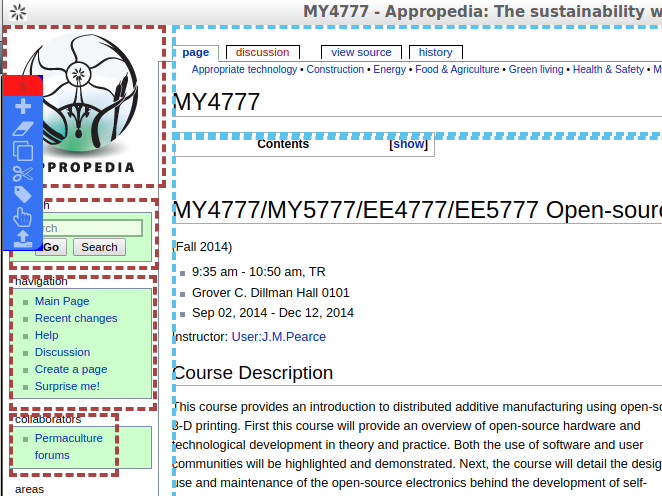
\includegraphics[width=250px]{new-mob.png}}
\caption{Nueva versi\'on de MoB}
\label{fig3}
\end{figure}

Como se mencionó anteriormente en la Sección II, en el trabajo de  Sanoja y Gancarski (2015) \cite{Sanoja:LIP6:2015,SanGan:SAC:2015} se presenta una versión prototipo de la herramienta de segmentación manual la cual se busca mejorar en este presente trabajo. En la Figura \ref{fig3} se puede observar que la nueva versión de la herramienta posee las siguientes características a diferencia de la antigua versión:
\begin{itemize}
\item El color de los bloques refleja el estado de los mismos y no el nivel de la segmentación, pues la segmentación es plana. En este ejemplo azul significa que está correcto y rojo que necesita atención. Se considera correcto verificando la granularidad, si tiene etiqueta, si no hay superposición de bloques, entre otras consideraciones menores.
\item Se restringe al usuario a realizar una segmentación plana, lo cual se considera deseable, a diferencia de la versión anterior la cual es propensa a segmentar en múltiples niveles.    
\item El panel de información ofrece mayor información sobre la granularidad presente y los bloques, además de los posibles errores o advertencias que puedan ocurrir. 
\item La caja de herramienta ocupa menos espacio al estar conformada únicamente de metáforas de las acciones, también es semi-transparente para poder observar el contenido que existe detrás.
\item Todas las acciones son llevadas a cabo únicamente con el ratón, sin tener que usar el teclado. 
\item Se ofrece la acción de ``cortar'' para poder separar bloques que se intersectan, y la acción ``seleccionar'' que permite obtener toda la información de un bloque en específico.  
\end{itemize}

\section{MoB API y MoB Repository}
\label{api_repo}
El MoB API y el MoB Repository están estrechamente relacionados, ya que, el MoB API no sólo ofrece servicios RESTful sino también actúa como backend del MoB Repository. A continuación se hace una descripción de las características más resaltantes de ambos y su finalidad en el sistema. 

\subsection{MoB API}
El desarrollo de la API se realizó con el lenguaje de programación Python v.3.5, apoyado con el microframework Flask v.0.12.2. Para la creación de la base de datos que va conectada a la API se utilizó el manejador de base de datos PostgreSQL v.10.1 junto con un componente llamado Postgis 2.4 para realizar las operaciones entre tablas.

En general, la API de MoB se divide en dos partes: todos los servicios RESTful que pueden ser ofrecidos a la Extensión MoB o a terceros y todas aquellas funciones que manejan el backend del Repositorio MoB.

A continuación se describen los servicios RESTful que son ofrecidos por la API, mientras que las funciones que manejan el backend del Repositorio de MoB se explicarán en la siguiente subsección. Los servicios ofrecidos son los siguientes:
\begin{itemize}
\item \textbf{Registrar usuario:} Permite registrar a un usuario en el sistema. Para completar el registro se le envía al usuario un enlace de activación a su correo. 

\item \textbf{Iniciar sesión:} Permite al usuario registrado (y activado) iniciar sesión en el sistema para hacer uso de sus funcionalidades. 

\item \textbf{Cerrar sesión:} Borra las \textit{cookies} de sesión existentes en el navegador y la sesión existente en el API. 

\item \textbf{Recuperar contraseña:} Permite al usuario recuperar su contraseña en caso de extravío. El sistema envía una combinación aleatoria de caracteres como contraseña temporal. Por medidas de seguridad las contraseñas se encuentran encriptadas por \textit{hash} en la base de datos. 

\item \textbf{Obtener colecciones:} Permite obtener una lista con los nombres de las colecciones y categorías de estas existentes en la base de datos del sistema.

\item \textbf{Obtener etiquetas:} Permite obtener una lista con los nombres de las etiquetas existentes en la base de datos del sistema.

\item \textbf{Obtener puntajes globales:} Permite obtener una lista con los mejores puntajes en cada una de las granularidades de una página Web específica.

\item \textbf{Obtener puntajes del usuario:} Permite obtener una lista con los puntajes en cada una de las granularidades de una página Web específica para un usuario determinado.

\item \textbf{Cargar segmentación:} Este es uno de los servicios más importante del API pues representa la base de todo el sistema. Permite cargar los resultados de una segmentación a la base de datos y los datos de la página Web, en caso de que sea la primera vez que se segmenta. Formando así lo que denominamos anteriormente como base de la verdad.

\item \textbf{Vista previa de segmentación:} Devuelve un \textit{canvas} con las figuras y etiquetas de los bloques segmentados para una segmentación en específica.

\item \textbf{Obtener segmentación en formato JSON:} Retorna un JSON con todos los datos de una segmentación en específica. 

\item \textbf{Obtener segmentación en formato V-PRIMA:} Retorna todos los datos de una segmentación en formato V-PRIMA. El formato V-PRIMA es un XML donde se especifican los bloques existentes en la segmentación y los enlaces, imágenes y textos existentes dentro de estos. Es una adaptación del formato V-DIFF a nuestro contexto \cite{Pehlivan:DEXA:2010}.

\item \textbf{Obtener segmentación en formato MoB HTML:} Retorna el HTML original con la información de la segmentación incluida. Se usan \emph{tags} personalizados, eg. $<block>$.

\item \textbf{Obtener página Web en formato WARC:} Devuelve la información de una página Web en formato WARC (Web ARChive). El formato WARC permite la concatenación de múltiples objetos de datos o recursos en un sólo archivo. Es utilizado para almacenar la información de páginas Web junto con sus recursos y metadata.

\end{itemize}

\subsection{Mob Repository}
El sitio Web MoB Repository se desarrolló haciendo uso del lenguaje de marcado HTML5, CSS3 y el lenguaje de programación Javascript. 
Usamos también el \textit{framework} \textit{JQuery}, principalmente para el comportamiento de las páginas y control de eventos. 
Todo esto del lado del cliente. 
Del lado del servidor está apoyado por el MoB API (Python y Flask) y la base de datos conectada a este (PostgreSQL y Postgis).

La finalidad del MoB Repository es ofrecerle a los usuarios del sistema una interfaz para que puedan visualizar las colecciones de segmentaciones manuales almacenadas en la base de datos. Ver las mejores segmentaciones manuales de cada página Web segmentada. 
A los usuarios administradores les permite administrar las etiquetas utilizadas en la segmentación, las colecciones y sus categorías, así como los roles de otros usuarios. 

\subsection{Creación de la Mejor Segmentación}

Como se mencionó en la introducción, definimos que para nuestro trabajo, según nuestra experiencia y los datos obtenidos, la mejor segmentación manual es aquella que contiene los bloques más populares en un conjunto de segmentaciones manuales.
Si la mayoría de usuarios han marcado un área de la página como un bloque, este se considerará popular.
Entonces tomamos los bloques más populares, creamos una nueva segmentación que los contenga, esta será considerada la mejor.

Al llevar a cabo la comparación, los bloques recibirán una serie de puntajes dependiendo de sus similitudes geométricas, con respecto a los otros bloques. 
Los puntajes de todos los bloques correspondientes a una misma segmentación podrán ser sumados dando la puntuación total de la segmentación. 
Esto quiere decir que mientras mayor sea el puntaje obtenido, mayor es el número de segmentaciones que la respaldan. 

Varios de estos atributos se nombran durante el proceso de comparación, por lo que aquí se presenta una leyenda de los mismos:
\begin{itemize}
\item \textbf{Identificador:} Un identificador arbitrario del bloque. 
\item \textbf{Geometría:} La geometría del bloque (área, ubicación y coordenadas del rectángulo asociado)
\item \textbf{Puntaje Geométrico:} La puntuación obtenida por similitudes geométricas. 
\item \textbf{Etiqueta:} La etiqueta que le fue asignada al bloque. 
\item \textbf{Puntaje Semántico:} La puntuación obtenida por similitudes semánticas (\emph{ie.} labels). 
\end{itemize}

El proceso de creación de la mejor segmentación consta de las siguientes 3 etapas: 
\begin{enumerate}
\item \textbf{Identificación de los bloques:} principalmente se deben identificar los bloques de la nueva segmentación a ser creada $S_{n+1}$. Se seleccionan en base a una comparación utilizando las $n$ segmentaciones ya almacenadas, $S_{1},...,S_{n} $. 
El proceso se puede describir en dos pasos: 
\begin{enumerate}
\item se fija un bloque $b_{k}^{n+1} \in S_{n+1}$, 
\item se compara contra todos los bloques en todas la segmentaciones pertinentes, $\forall b_{j}^{i} \in S_i$ con $i \in [1,n]$ en las demás segmentaciones. 
Se considera una tolerancia basada en la Distancia Hausdorff \footnote{La distancia Hausdorff es la mayor de todas las distancias existentes desde un punto en un conjunto hasta el punto más cercano en otro conjunto.} entre $b_{k}^{n+1}$ y un $b_{j}^{i} $. 
Si la distancia es menor o igual a T \footnote{generalmente $T=30px$} se considera que ambos bloques son similares y el $b_{j}^{i}$  tendría el mismo identificador que $b_{k}^{n+1}$.  
 \end{enumerate}
\item \textbf{Contabilización de puntos:} para complementar el paso anterior, se contabilizan todos los bloques bajo un mismo identificador, para obtener el \textit{puntaje geométrico}. Después, dentro del mismo \textit{pool} de bloques con el mismo identificador se contabilizan todos los que posean las mismas etiquetas, de esta forma obtener el \textit{puntaje semántico}. 
En la Figura \ref{fig:geom} se observa el cálculo del \textit{puntaje geométrico}. El bloque $b_{1}^{1}$ tiene equivalentes en las tres segmentaciones restantes. 
Esto contabiliza 4 ocurrencias en el conjunto de segmentaciones.
Para el bloque $b_{1}^{4}$ tiene correspondencia en dos de las segmentaciones restantes.
Finalmente se suman las ocurrencias y se obtiene el puntaje geométrico.
Este cálculo se realiza cada vez que se incorpora una nueva segmentación de una página.

\begin{figure}[!h]
\centering
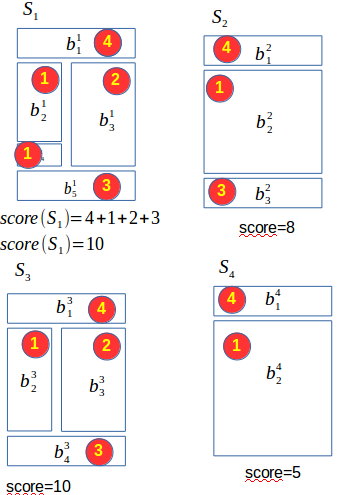
\includegraphics[width=230px]{mob-best.png}
\centering\caption{Ejemplo de puntajes geométricos}
\label{fig:geom}
\end{figure}

En la Figura \ref{fig:lab} se muestra un ejemplo para el cálculo del \textit{puntaje semántico}.
Se basa en la coincidencia geométrica y adicionalmente que la etiqueta de los bloques coincidan.
En el ejemplo se puede observar para la segmentación $S_1$ las siguientes etiquetas: HDADF (corto para \textit{header}, \textit{aside}, \textit{article}, \textit{aside} y \textit{footer}, respectivamente).
La segmentación $S_1$ tiene el mayor \textit{puntaje semántico}. Es un fuerte candidato para ser incorporado

\begin{figure}[!h]
\centering
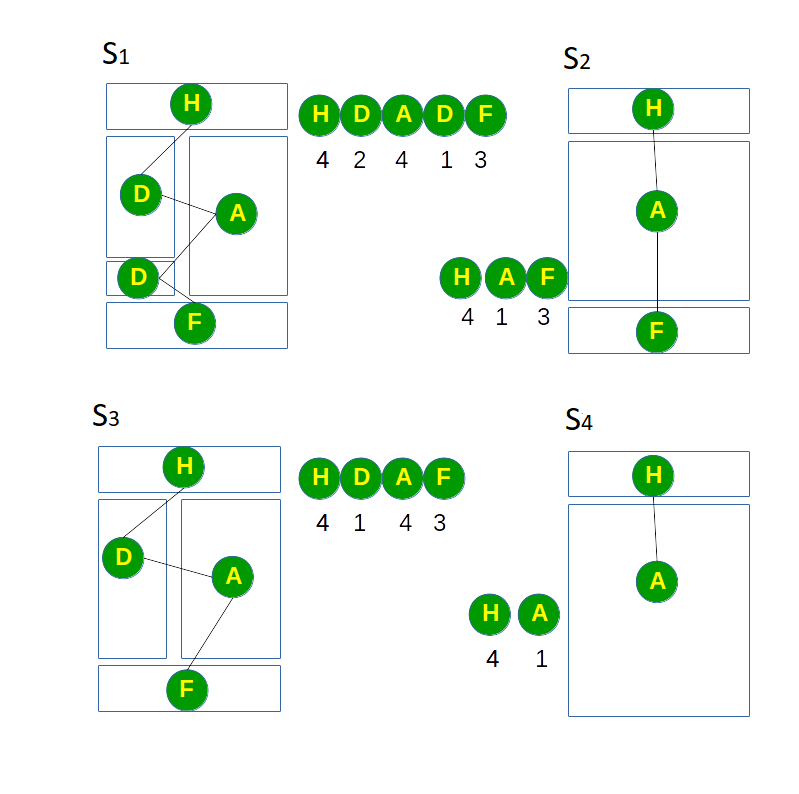
\includegraphics[scale=0.4]{mob-best-label-2.png}
\centering\caption{Ejemplo de puntajes semánticos}
\label{fig:lab}
\end{figure}

\item \textbf{Creación de la mejor segmentación:} para crear la mejor segmentación se incluyen todos aquellos bloques (uno por cada identificador) cuyo \textit{puntaje geométrico} sea mayor que el 50\% del número de segmentaciones realizadas, esto garantiza que la mayoría de los usuarios opina que ese bloque debe existir. Dicho bloque poseerá la etiqueta más utilizada para ese bloque, es decir, se busca entre los de un mismo identificador la etiqueta que tenga el mayor \textit{puntaje semántico}. En el ejemplo mostrado en la Figura \ref{fig:lab} el bloque $b_{1}^{1}$ tendría asociada la etiqueta H la cual es la más popular para esa área de la página.
\end{enumerate}

\section{Verificación del Sistema}
\label{resultados}
Para verificar el sistema desarrollado, se llevaron a cabo dos pruebas de aceptación, una funcional y otra no funcional, las cuales se describirán a continuación. 

\subsection{Prueba Funcional}
Para comprobar la funcionalidad del sistema, se realiza una prueba de caja negra. 
Se busca comprobar si el sistema se comporta como es esperado según las funciones que debe realizar. Tal es el caso en la MoB Extension de insertar, modificar y eliminar bloques. Al modificar se verifica la unión y separación de bloques. En el MoB API la gestión de segmentaciones (\emph{eg} agregar, visualizar), así como la creación de la mejor segmentación. Y para el MoB Repository observar que las segmentaciones y páginas estén completas y con todas sus dependencias.
%
La técnica utilizada es principalmente la observación, dada la experiencia con los datos manejados, de manera satisfactoria.

\subsection{Prueba no Funcional}
Las pruebas no funcionales se enfocaron en asegurar si la herramienta es usable o no. Específicamente la herramienta MoB Extension, para esto se evalúa la reacción de 5 individuos ante el sistema. Se observó las reacciones de los participantes mientras completan 2 objetivos planteados y finalmente se les dio un cuestionario para responder según su experiencia. Cabe destacar que la herramienta está orientada a usuarios de 13 años en adelante, con inexistentes, bajos, intermedio o avanzados conocimientos en segmentación de páginas Web. 
En la Figura \ref{fig:nofunc} se muestra un resultado de ejemplo del formulario. 
Dada la extensión del formato de los datos, no se muestran en este documento los gráficos completos, pero pueden ser consultados en \cite{GARCIA2018}. En la misma figura puede observarse la pregunta del cuestionario: ¿cuánto tiempo se tomó en realizar el segundo objetivo? teniendo que el 40\% le tomó entre 5 y 10 minutos, mientras que el 60\% lo finalizó en menos de 5 minutos.
%
Respuestas como estas nos permiten tener la confianza que se ha mejorado la usabilidad substancialmente. Tomando en consideración que los usuarios de la versión anterior debían tener un \emph{background} muy avanzado para poder usar la herramienta.

\begin{figure}[!h]
\centering
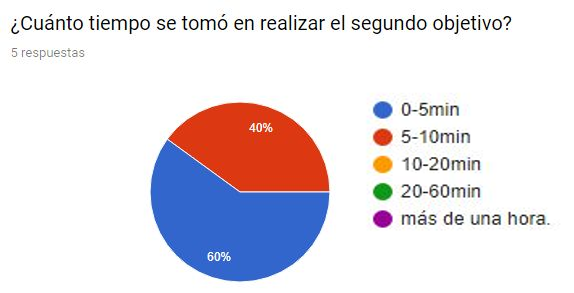
\includegraphics[scale=0.4]{verif.png}
\centering\caption{prueba no funcional: Pregunta 5 del cuestionario}
\label{fig:nofunc}
\end{figure}

\begin{itemize}
\item Realizar una segmentación manual sobre la página Web: https://wiki.apache.org/httpd/RedirectSSL.
\item Visitar el Repositorio de MoB y observar la segmentación realizada.
\end{itemize}

En conclusiones generales, basándose en las respuestas obtenidas del cuestionario, los comentarios hechos por los participantes y el comportamiento observado de los mismos, se tiene que:
\begin{itemize}
\item El sistema en general presenta un aspecto estético agradable para los usuarios. 
\item La herramienta de segmentación permite a los usuarios inexpertos realizar segmentaciones rápidamente sobre una página Web, de una forma sencilla.
\item La navegación general del Repositorio MoB es entendible, sin embargo cuando se debe profundizar, buscar segmentaciones específicas, el usuario debe invertir un poco de tiempo en entender la lógica de la navegación. 
\end{itemize}
Se puede considerar que el sistema MoB es usable, sin embargo, algunos usuarios requieren una breve inducción. 

\section{Conclusiones y Trabajos a Futuro}
\label{conclusiones}
Durante el desarrollo de la herramienta de segmentación manual (Extensión de MoB), se presentó uno de los retos más grandes del proyecto. Se requirió no sólo que cumpliese con su misión de segmentar manualmente la página Web, sino mejorar significativamente la usabilidad.
Las pruebas de caja negra y usabilidad permitieron validar los objetivos iniciales de la herramienta. Se logró reducir la complejidad de una tarea tediosa y propensa a errores mediante la automatización.

En cuanto al repositorio de MoB, el mayor reto fue lograr una forma comprensible de ordenar toda la información sobre las páginas Web y sus segmentaciones. Después de realizar las pruebas de caja negra se evidenció que el repositorio funcionaba como se esperaba. Aun algunos usuarios encontraban difícil la navegación en el sitio. Esta información recopilada puede ser tomada en cuenta para las mejoras a futuro que se vayan a realizar sobre el sistema. 

Entre los retos presentados en el desarrollo del API de MoB se encontraba: el poder desarrollar todos los servicios pertinentes de una forma modular. Presentar estructuras de respuesta que fuesen fácil de comprender y manejar, en especial la estructura de bloques que se debe usar para la carga de los datos de la segmentación. 
Se incluye una parte de la implementación en background para poder detectar una nueva segmentación e invocar el proceso de cálculo de la mejor segmentación manual. Reducir el tiempo de respuesta de este proceso fue un reto, y que diera respuesta en un tiempo aceptable. Esto fue resuelto sin contratiempos incluyendo una base de datos con extensiones geográficas como \textit{Posgis}. De esta forma el análisis de comparar los diferentes bloques se realizo de manera rápida y eficaz.

Este proyecto comenzó con la idea de desarrollar una herramienta para ayudar en el desarrollo de otros proyectos. Sin embargo, a lo largo del desarrollo se fueron extendiendo las funcionalidades principales y añadiendo funcionalidades adicionales a los elementos principales del sistema, reforzando la funcionalidad y permitiendo la evolución del mismo. Como resultado tenemos un sistema bastante completo en donde se pueden realizar segmentaciones manuales,  incluir segmentaciones hechas por algoritmos y ser almacenadas. La información de las segmentaciones puede ser mostrada a través de una interfaz Web (Repositorio MoB), y en el caso de las segmentaciones manuales, pueden ser analizadas y obtener ese elemento que representa la razón principal por la cual se realiza este trabajo, la mejor segmentación manual. 


Para finalizar, la solución presentada permite incrementar la cantidad de páginas existentes en el repositorio \footnote{http://bom.ciens.ucv.ve/repo y https://mob.ciens.ucv.ve}, que hasta el momento posee cerca de 60 p\'aginas realizadas con el prototipo de MoB. 
Durante la realizaci\'on de las pruebas de la nueva versi\'on pudimos observar que agregar una nueva p\'agina manualmente segmentada promete ser menos complejo.
Esto ayuda al equipo de investigaci\'on a tener un dataset cada vez m\'as completo.

\subsection{Trabajos Futuros}

La inclusión de otros formatos de exportación para las segmentaciones sería una buena actualización.

Según los resultados arrojados por la prueba de usabilidad, el Repositorio MoB presenta una navegación que puede resultar algo confusa para algunos usuarios, es por eso que se propone como un trabajo a futuro la implementación de una navegación más intuitiva. 
Este tipo de retroalimentación nos permitirá acelerar la conformación de la base referencial.

Además, es importante destacar que la extensión actual funciona únicamente para el navegador Chrome/Chromium  es por eso que se plantea un trabajo a futuro donde se adapte dicha extensión para funcionar en una mayor variedad de navegadores (Firefox, Safari, Opera, entre otros).

Esta nueva versión permite incrementar la cantidad de usuarios participantes. Esto implica a corto plazo que se debe mejorar el MoB API para trabajar de manera concurrente en un ambiente de alto desempeño.

\bibliographystyle{ieeetr}
\begin{thebibliography}{10}

\bibitem{Zhu:18:WD}
Y.~Zhu, ``{W3C} dom {4.1},'' {W3C} working draft, W3C, Feb. 2018.
\newblock https://www.w3.org/TR/2018/WD-dom41-20180201/.

\bibitem{Sanoja:LIP6:2015}
A.~Sanoja, {\em Web Page Segmentation, Evaluation and Applications}.
\newblock PhD thesis, Universit{\'e} Pierre et Marie Curie-Paris VI,
  {\url{https://hal.inria.fr/tel-01128002/}}, 2015.

\bibitem{SanGan:SAC:2015}
A.~Sanoja and S.~Gan{\c{c}}arski, ``Web page segmentation evaluation,'' in {\em
  Proceedings of the 30th Annual ACM Symposium on Applied Computing},
  pp.~753--760, ACM, 2015.

\bibitem{Cai:APWEB:2003}
D.~Cai, S.~Yu, J.-R. Wen, and W.-Y. Ma, ``Extracting content structure for web
  pages based on visual representation,'' in {\em Proceedings of the 5th
  Asia-Pacific Web Conference on Web Technologies and Applications}, APWeb'03,
  (Xian, China), pp.~406--417, Springer-Verlag, 2003.

\bibitem{liu2011segmenting}
X.~Liu, H.~Lin, and Y.~Tian, ``Segmenting webpage with gomory-hu tree based
  clustering.,'' {\em JSW}, vol.~6, no.~12, pp.~2421--2425, 2011.

\bibitem{uzun2013hybrid}
E.~Uzun, H.~V. Agun, and T.~Yerlikaya, ``A hybrid approach for extracting
  informative content from web pages,'' {\em Information Processing \&
  Management}, vol.~49, no.~4, pp.~928--944, 2013.

\bibitem{Chakrabarti:WWW:2008}
D.~Chakrabarti, R.~Kumar, and K.~Punera, ``A graph-theoretic approach to
  webpage segmentation,'' in {\em Proceedings of the 17th international
  conference on World Wide Web}, (Beijing, China), pp.~377--386, ACM, 2008.

\bibitem{10.1145/3326457}
Z.~Jiang, H.~Yin, Y.~Wu, Y.~Lyu, G.~Min, and X.~Zhang, ``Constructing novel
  block layouts for webpage analysis,'' {\em ACM Trans. Internet Technol.},
  vol.~19, July 2019.

\bibitem{kiesel-etal-2017-wat}
J.~Kiesel, H.~Wachsmuth, K.~Al-Khatib, and B.~Stein, ``{WAT}-{SL}: A
  customizable web annotation tool for segment labeling,'' in {\em Proceedings
  of the Software Demonstrations of the 15th Conference of the {E}uropean
  Chapter of the Association for Computational Linguistics}, (Valencia, Spain),
  pp.~13--16, Association for Computational Linguistics, Apr. 2017.

\bibitem{bjdmnmd2019}
J.~Blustein, N.~R. Di~Matteo, and D.~Macrini, ``Designing experiments to
  compare web page segmenters,'' in {\em Proceedings of the 2nd International
  Workshop on Human Factors in Hypertext}, pp.~27--29, 2019.

\bibitem{krh2015}
R.~Kreuzer, J.~Hage, and A.~Feelders, ``A quantitative comparison of semantic
  web page segmentation approaches,'' in {\em International Conference on Web
  Engineering}, pp.~374--391, Springer, 2015.

\bibitem{Sanoja:ICMCS:2014}
A.~Sanoja and S.~Gan{\c c}arski, ``Block-o-matic: A web page segmentation
  framework,'' in {\em International Conference onMultimedia Computing and
  Systems (ICMCS)}, (Marrakesh, Moroco), pp.~595--600, April 2014.

\bibitem{Pehlivan:DEXA:2010}
Z.~Pehlivan, M.~Ben-Saad, and S.~Gan\c{c}arski, ``Vi-diff: Understanding web
  pages changes,'' in {\em Proceedings of the 21st International Conference on
  Database and Expert Systems Applications: Part I}, DEXA'10, (Berlin,
  Heidelberg), pp.~1--15, Springer-Verlag, 2010.

\bibitem{GARCIA2018}
J.~P. Garcia, ``Desarrollo de una herramienta interactiva para la construcción
  de un ``ground truth'' de segmentaciones de páginas web,'' tech. rep.,
  Escuela de Computación. Universidad Central de Venezuela, 2018.

\end{thebibliography}
%\bibliography{references}


% that's all folks
\end{document}


